% !TEX encoding = UTF-8 Unicode
% !TEX spellcheck = en_US

\documentclass[graybox,vecphys]{svmult}

\usepackage{makeidx} % allows index generation
\usepackage{graphicx}
\graphicspath{{./figures/}}
\usepackage{multicol} % used for the two-column index
\usepackage[bottom]{footmisc} % places footnotes at page bottom

%%% Custom commands
\newcommand{\bm}[1]{\boldsymbol{#1}}
\newcommand{\rotmat}[2]{{{ }^{#1}\boldsymbol{R}}_{#2}}
\newcommand{\ks}[1]{{(\mathrm{CS})_{#1}}}
\newcommand{\ortvek}[4]{{ }_{(#1)}{\boldsymbol{#2}}^{#3}_{#4} }
% Commands for symbol of the residual (full and reduced)
\newcommand{\Res}[0]{\vec{\delta}}
\newcommand{\ResR}[0]{\vec{\psi}}

%%% custom packages
\usepackage[T1]{fontenc}
\usepackage[utf8]{inputenc}
\usepackage{amsmath,amsfonts}
\usepackage{paralist} % for compactitem
\usepackage{siunitx}
\usepackage{url}
\usepackage{newtxtext}
\usepackage[varvw]{newtxmath} % selects Times Roman as basic font
\makeindex 

\begin{document}

\title*{Geometric Model for Serial-Chain Robot Inverse Kinematics in Case of Two Translational DoF, Spatial Rotation and Functional Redundancy}
\author{Moritz Schappler \and Tobias Blum \and Tim-David Job}
\institute{%
All authors are with the Leibniz University Hannover, Institute of Mechatronic Systems. \email{moritz.schappler@imes.uni-hannover.de}}

\titlerunning{Inverse Kinematics for Two Translational DoF with Spatial Rotation}
\authorrunning{M. Schappler et al.}

\maketitle
\vspace{-2.7cm} % space above is reserved for author affiliations. Take the space since the one affiliation is on the footer
\abstract{% 10-15 lines long
Geometric formulations for the inverse kinematics problem (IKP) in robotics are often set up in the full Cartesian space of three translational and three rotational coordinates (3T3R).
When transferring this to tasks with spatial rotation
like 3T2R, 2T3R or 2T2R, the result is usually not defined in a minimal set of independent coordinates.
Removing the excluded operational space coordinates completely from the expressions is interesting from a theoretical point of view and simplifies further calculations.
This can be achieved by formulating a 2R residual using the $Z$-$Y'$-$X''$ Tait-Bryan angles and a 2T residual derived by the projection of the pointing direction on a plane.
In this paper, the minimal-coordinate IKP is derived for 2T2R and 2T3R tasks on position level with application to a gradient-projection scheme.
Limitations of the redundant coordinate are considered within the nullspace.
} 

\keywords{Serial-link robot, Inverse kinematics, Functional redundancy, Geometric model, Nullspace projection, 2T2R, 2T3R, Coordinate inequality constraint}

\vspace{-0.5cm}
\section{Introduction and State of the Art}
\vspace{-0.1cm}
\label{sec:introduction}

The inverse kinematics of robot manipulators in tasks with reduced degrees of freedom (DoF) has been investigated in the context of \emph{functional redundancy}, where operational space and joint space have more DoF than the task space \cite{SciaviccoSic2000}.
Some tasks with axis-symmetric tools like welding \cite{Baron2000,HuoBar2008} or drilling \cite{ZanchettinRocRobJoh2011,ZhuQuCaoYan2013} require three translational and two rotational DoF (3T2R), where six-axis robots are redundant.

In some applications, the process is also \emph{independent of the feed} in the tool axis' direction. 
This results in a task with five DoF with full orientation (2T3R) or four DoF with rotational symmetry (2T2R), which can lead to one or two redundant DoF. 
In waterjet cutting the jet can have an effective cutting range of several centimeters \cite{BahlsFroHelDeu2017}. 
The laser target acquisition task e.g. allows arbitrary motion in beam direction \cite{ChenMcIYi2003}.
Other laser appliances like laser cutting \cite{DolguiPas2009} or remote laser welding \cite{ErdoesKarKem2015} can have a variable distance with a focus area or an adjustable focus point.
Further examples are drilling with a dedicated feed axis of the drilling tool \cite{KoblerKotLexMaj2014}, spraying with a range of distance \cite{FromGra2010} or the usage of a camera with a specific depth of field \cite{GuetaCheChiAra2011}. 
It should be noted that in most of these 2T applications, the feed can not be disregarded as for the 2R case, but merely has to be \emph{limited to an acceptable range} \cite{GuetaCheChiAra2011}.
A related case are 2T constraints in the remote center of motion (RCM) problem \cite{SadeghianZokJaz2019, SandovalPoiVie2017}.
%
Exemplary \emph{2T applications specifically of parallel mechanisms} are 2T3R medical needle holders \cite{KumarPicBay2014}, laser satellite tracking (implemented as 3T2R in \cite{ChenMcIYi2003}), 2T2R oscillating screens \cite{YeFanGuoQu2014} or simulation of a 2T3R spinal cord in bionics \cite{ZhuHuaZha2009}.

The solution of the inverse kinematic problem (IKP) with functional redundancy can be obtained with the well-established \emph{nullspace-projection method} \cite{SciaviccoSic2000}. 
A requirement to use the method is the proper construction of the IK residual and the IK Jacobian.
One way is to add a virtual joint into the kinematic structure and to augment the manipulator Jacobian by one column \cite{Baron2000}. 
By adding a virtual prismatic joint the 3T2R task from \cite{Baron2000} can be transferred to a 2T2R task like in \cite{ErdoesKarKem2015} or for the RCM problem in combination with an RCM-constrained Jacobian in \cite{SadeghianZokJaz2019}.
The \emph{augmentation approach} has the drawback that it has a higher computational cost and can lead to an ill-conditioned Jacobian \cite{HuoBar2008}.
The need of a \emph{minimal-coordinate approach} is emphasized for the RCM problem in \cite{SandovalPoiVie2017}.
Another option to adapt the Jacobian is to reduce it instead of augmenting it by removing a row of the ``task frame Jacobian'' \cite{Zlajpah2017}. 
\emph{Reducing the Jacobian} requires calculating the full residual and Jacobian first and removing the redundant row subsequently \cite{SchapplerTapOrt2019a}. 

Further solutions for the functional redundancy are based on the orthogonal decomposition of the twist \cite{HuoBar2005} or constructing a cone or pyramid with a range of tolerances for tilt angles and positions on the tool axis \cite{FromGra2010}.
Another approach uses a \emph{functional relationship between task DoF and redundant DoF} for an optimized performance index via Monte-Carlo simulation \cite{ZanchettinRocRobJoh2011}.
Identifying the functional relationship requires pre-defining a functional space.
For the considered 2T2R case with two redundant DoF a \emph{closed-form solution} is harder to obtain, if possible at all.
%
\emph{Cascaded optimization} utilizes an inner loop that solves the standard IK problem and an outer loop optimizing the performance index \cite{ZhuQuCaoYan2013}. 
%
Cascaded optimization and global optimization in general have higher computational cost and do not exploit the \emph{nullspace-projection method}, which is favorable due to \emph{local optimality} and efficiency, provided a feasible formulation is chosen. 
In \cite{MoeAntTeePet2016} e.g. only a scalar potential is used as a constraint for a cone-like task similar to 2T2R, termed ``field of view''. 
This leads to issues with the differentiability \cite{MoeAntTeePet2016} and therefore with IK convergence.

Despite their occasional occurrences in literature, the kinematics of tasks with 2T3R and 2T2R DoF are not \emph{systematically investigated for functional redundancy} yet and methods for a general modeling of these tasks are sparse. 
Further, the problem is mostly formulated on \emph{velocity level} which requires attention when handling the nonlinear orientation residual, since the residual's Jacobian is not  the differential kinematics Jacobian.
In this paper a general minimal-coordinate geometric approach for the \emph{position-level} IKP for 2T3R and 2T2R tasks is presented. 
The focus lies on local optimization, as motivated above.
%
The contributions of this paper are:
\begin{compactitem}
\item a general kinematic modeling approach for the IKP of 2T3R and 2T2R tasks,
\item an application to the inverse kinematics of serial robots with functional redundancy and redundant coordinate limitations, shown by a simulation example.
\end{compactitem} 

% Layout: This should still be on page 2!
The outline of this paper is as follows. In Sect.\,\ref{sec:model} the proposed kinematic modeling approach for a serial chain is shown. 
The application to inverse kinematics and the resolution of functional redundancy is given in Sect.\,\ref{sec:inverse}. 
Section\,\ref{sec:simulation} demonstrates the results of the simulation examples and Sect.\,\ref{sec:conclusion} concludes the paper.

\section{Inverse Kinematic Model for Serial Chains} % Layout: begin of page 3
\label{sec:model}

\begin{figure}[b]
\vspace{-0.3cm}
\centering
\input{figures/kinematic_principle.pdf_tex}
\vspace{-0.3cm}
\caption{(\textbf{a}) Geometric approach for the IK's position residual and (\textbf{b}) orientation residual}
\label{fig:geometry_sketch}
\end{figure}

For robots in 2T2R and 2T3R tasks one translational DoF needs to be removed from the kinematic equations to obtain an expression of minimal dimension. 
This DoF is defined to be the displacement along the end effector's $z$ axis.
% 
The established formulation for the translational part of the inverse kinematics (IK) residual that relates the robot's joint coordinates $\vec{q}$ and operational space coordinates $\vec{x}$ is
%
\vspace{-0.1cm}
\begin{equation}
\label{eq:Phi_t_3T3R}
{\tilde{\Res}_\mathrm{t}(\vec{q},\vec{x})} 
= 
\ortvek{0}{r}{}{DE}
=
-{_{(0)}\vec{r}_D} + {_{(0)}\vec{r}_E}(\vec{q}) = -\vec{x}_{\mathrm{t}} + {_{(0)}\vec{r}_E}(\vec{q}) ~\in {\mathbb{R}}^{3}
\vspace{-0.1cm}
\end{equation}
%
with $\vec{x}^\transp
=
\begin{bmatrix}
\vec{x}_{\mathrm{t}}^\transp & 
\vec{x}_{\mathrm{r}}^\transp
\end{bmatrix}
= 
\begin{bmatrix}
r_{0D,x} & 
r_{0D,y} & 
r_{0D,z} & 
\varphi_x &
\varphi_y &
\varphi_z
\end{bmatrix}
\in {\mathbb{R}}^{6}$ and $\vec{x}_{\mathrm{r}}$ as Tait-Bryan angles.
% 
Coordinate systems are defined for the robot base $\ks{0}$, the actual end effector pose $\ks{E}$ and the desired pose $\ks{D}$, expressed with $\vec{x}$.
The residual (\ref{eq:Phi_t_3T3R}) is not feasible for the 2T case since it would correspond to an exact position adjustment.
To obtain translational redundancy, new coordinates must be chosen that allow an elimination of the redundant DoF in the residual.
The goal is to choose the coordinates $\vec{x}_\mathrm{t}$ and $\vec{x}_\mathrm{r}$ so that they can be reduced via selection matrices to 
$
\vec{y}_{\mathrm{t}}
=
\vec{P}_{y,\mathrm{t}}\,\vec{x}_{\mathrm{t}}$
for the 2T case and
%\quad \mathrm{and} \quad
$
\vec{y}_{\mathrm{r}}
=
\vec{P}_{y,\mathrm{r}}\,\vec{x}_{\mathrm{r}}
$
for the 2R case.
%
By stacking the translational and rotational coordinates the combinations 2T2R and 2T3R (and also 3T2R or 3T3R) can be created. 

In this approach the translational task \emph{minimal} coordinates are chosen as 
%
\vspace{-0.1cm}
\begin{equation}
\label{eq:minimalkoordinaten_2T}
\vec{y}_{\mathrm{t}}
=
\begin{bmatrix}
r_{0D',x}  & r_{0D',y}
\end{bmatrix}^\transp
=
\vec{P}_{y,\mathrm{t}}
\begin{bmatrix}
r_{0D',x} & 
r_{0D',y} & 
{\lambda_{D'}}
\end{bmatrix}^\transp
\in {\mathbb{R}}^{2},
\vspace{-0.1cm}
\end{equation}
%
where the index $D'$ in $r_{0D',x}$ and $r_{0D',y}$ refers to the intersection of the $z$ axis of $\ks{D}$ with the $x$-$y$ plane of $\ks{0}$ shown in Fig.~\ref{fig:geometry_sketch}a and $\lambda_{D'} = {_{(D)}r_{DD',z}}$ is the distance to this intersection point which is derived in the following. 

The point $E'$ is obtained similarly from $\ks{E}$ by setting up a line equation %${\vec{g}(\vec{q})}$ 
%
\vspace{-0.1cm}
\begin{equation}
\label{eq:equation_system}
{\vec{g}(\vec{q})}
={_{(0)}\vec{r}_E(\vec{q})}+ {\lambda{_{(0)}\vec{e}_{z}^{E}}(\vec{q})}
\vspace{-0.1cm}
\end{equation}
%
from the vector of location ${_{(0)}\vec{r}_E(\vec{q})}$ in the direction of the $z$ axis $\vec{e}_{z}^{E}(\vec{q})$ of $\ks{E}$.
%
The intersection
${_{(0)}\vec{r}_{E'}}
$
of the line in (\ref{eq:equation_system}) with the $x$-$y$ plane of $\ks{0}$ is obtained by
%
\vspace{-0.1cm}
\begin{equation}
\label{eq:lambda_Edash}
{\lambda(\vec{q})} 
= 
{\lambda_{E'}(\vec{q})} 
= 
\left(0 - r_{0E,z}(\vec{q})\right)/{e_{z,z}^E}(\vec{q}) 
= 
-r_{0E,z}(\vec{q}) / e_{z,z}^E(\vec{q}).
\vspace{-0.1cm}
\end{equation}

Inserting ${\lambda_{E'}}$ in $\vec{g}(\vec{q})$ gives ${_{(0)}\vec{r}_{E'}}$, which is also sketched in Fig.~\ref{fig:geometry_sketch}a.
The variable ${\lambda_{E'}}$ can be understood as the distance from $\ks{E}$ to $E'$. 

% Layout: The page should end with the sentence above

With the new coordinates corresponding to (\ref{eq:minimalkoordinaten_2T}), the translational residual 
%
\vspace{-0.1cm}
\begin{equation}
\label{eq:Phit}
\Res_\mathrm{t}(\vec{q},\vec{x})
=
\begin{bmatrix}
{-}r_{0D',x}(\vec{x}) {+} r_{0E',x}(\vec{q}) ,\enspace &
{-}r_{0D',y}(\vec{x}) {+}r_{0E',y}(\vec{q}) ,\enspace &
{-} {\lambda_{D'}(\vec{x})} {+} {\lambda_{E'}(\vec{q})}
\end{bmatrix}^\transp
\vspace{-0.1cm}
\end{equation}
%
is now defined.
The reduced residual for 2T tasks can be obtained through
%
\vspace{-0.1cm}
\begin{equation}
\label{eq:Psit_2T}
\ResR_\mathrm{t}(\vec{q},\vec{y}) = 
\begin{bmatrix}
    1 & 0 & 0  \\ 
    0 & 1 & 0
\end{bmatrix}
 \Res_\mathrm{t}(\vec{q},\vec{x})
 =\vec{P}_{\ResR,\mathrm{t}} \Res_\mathrm{t}(\vec{q},\vec{x})
 ~\in {\mathbb{R}^2}.
 \vspace{-0.1cm}
\end{equation} 
%
The peculiarity of the kinematic model lies in the \emph{sole dependency on the reduced coordinates} $\vec{y}$.
For the solution of the IKP shown in Sect.\,\ref{sec:inverse} the gradient of the residual w.r.t. $\vec{q}$ is needed.
It follows by partial derivation (and by ignoring the third row) to
%
\vspace{-0.1cm}
\begin{align}
{\frac{\partial}{\partial\vec{q}}\ResR_\mathrm{t}}(\vec{q},\vec{x}) 
&= 
\vec{P}_{\ResR,\mathrm{t}} {\Big(\frac{\partial}{\partial\vec{q}}{_{(0)}\vec{r}_{0E'}(\vec{q})}\Big)}
= \vec{P}_{\ResR,\mathrm{t}}
{\Big(\frac{\partial}{\partial\vec{q}}{_{(0)}\vec{r}_{0E}(\vec{q})}} + 
{\frac{\partial}{\partial\vec{q}}\big({\lambda_{E'}(\vec{q})}{_{(0)}\vec{e}_{z}^E}(\vec{q})\big)\Big)} \nonumber \\
&= 
\vec{P}_{\ResR,\mathrm{t}}
{\Big(\frac{\partial}{\partial\vec{q}}{_{(0)}\vec{r}_{0E}(\vec{q})}} + 
{\frac{\partial{\lambda_{E'}(\vec{q})}}{\partial\vec{q}}}{_{(0)}\vec{e}_{z}^E}(\vec{q}) +
{{\lambda_{E'}(\vec{q})}\frac{\partial{_{(0)}\vec{e}_{z}^E}(\vec{q})}{\partial\vec{q}}\Big)}.
\label{eq:Phi_grad_2T2R_2}
\vspace{-0.1cm}
\end{align}
%
Since ${\lambda_{E'}(\vec{q})}$ from (\ref{eq:lambda_Edash}) is the quotient of  ${f_\mathrm{1}(\vec{q})} = {-{r_{0E,z}(\vec{q})}}$ and ${f_\mathrm{2}(\vec{q})} = {e_{z,z}^E(\vec{q})}$, dependent on $\vec{q}$, it's partial derivative is calculated by the quotient rule for differential calculus.
%
The term ${\partial{\vec{e}_{z}^E}(\vec{q})}/{\partial\vec{q}}$ in $f_\mathrm{2}$ can be obtained either by symbolic derivation using computer algebra systems or by a relation with the rotational part of the geometric Jacobian, which can be derived with the methods from \cite{SchapplerTapOrt2019a}. 
The rotational residual is calculated as in \cite{SchapplerTapOrt2019a} using $Z$-$Y'$-$X''$ Tait-Bryan angles
%
\vspace{-0.1cm}
\begin{equation}
\Res_{\mathrm{r}}(\vec{q},\vec{x})
=
\vec{\alpha}\left(\rotmat{D}{E}(\vec{q},\vec{x}_{\mathrm{r}})\right)
=
\vec{\alpha}\left(\rotmat{0}{D}^\transp (\vec{x}_{\mathrm{r}})\rotmat{0}{E}(\vec{q})\right)
=[\alpha_z,\alpha_y,\alpha_x]^\transp
~\in {\mathbb{R}^3}.
\vspace{-0.1cm}
\end{equation}
%
The series of elementary rotations is depicted in Fig.~\ref{fig:geometry_sketch}b.
By explicitly adding two intermediate frames $\ks{A1}$ and $\ks{A2}$ that share the same $z$ axis with the desired frame $\ks{D}$, the purpose of this angle convention becomes apparent. 
Since the rotation around this axis is the redundant DoF, these frames with elementary rotations $\varphi_z$ and $\alpha_z$ can be omitted for the reduced residual, which is sketched by the dashed line to $\ks{A2}$.
%
Analogously to (\ref{eq:Psit_2T}), multiplying a permutation matrix  leads to the reduced residual $\ResR_\mathrm{r}(\vec{q},\vec{y}) = \vec{P}_{\ResR,\mathrm{r}} \Res_{\mathrm{r}}(\vec{q},\vec{x})~\in {\mathbb{R}^2}$ for 2R tasks. 
For the derivation of the gradient $\ResR_{\mathrm{r},\partial \vec{q}}  = \partial \ResR_\mathrm{r} / \partial \vec{q}$ and details of this approach refer to \cite{SchapplerTapOrt2019a,SchapplerTapOrt2019}. 

Similar to the coordinate definitions $\vec{y}$ and $\vec{x}$, the full residual
$
\ResR(\vec{q},\vec{y})^\transp = \begin{bmatrix}
(\vec{P}_{\ResR, \mathrm{t}}\Res_\mathrm{t}(\vec{q},\vec{x}))^\transp &
(\vec{P}_{\ResR, \mathrm{r}}\Res_\mathrm{r}(\vec{q},\vec{x}))^\transp
\end{bmatrix}
$
is obtained by stacking the translational and rotational residual in any combination depending on the task DoF (2T2R, 2T3R, ...).
This is done by choosing the according permutation matrix, e.g. by $\vec{P}_{\ResR, \mathrm{t}}{=}\vec{P}_{\ResR, \mathrm{2T}}$, from 
%
\vspace{-0.1cm}
\begin{equation}
\vec{P}_{\ResR, \mathrm{3T}}=\bm{I}_3
,\quad
\vec{P}_{\ResR, \mathrm{2T}}=
\begin{bmatrix}
1 & 0 & 0  \\ 
0 & 1 & 0
\end{bmatrix}
,\quad
\vec{P}_{\ResR, \mathrm{3R}}=\bm{I}_3
,\quad
\vec{P}_{\ResR, \mathrm{2R}}=
\begin{bmatrix}
0 & 1 & 0  \\ 
0 & 0 & 1
\end{bmatrix}.
\vspace{-0.1cm}
\end{equation}
%
The constraint/residual definition above can be interpreted as a generalized formal description of an \emph{equality task} for the task coordinates $\vec{y}$, as e.g. discussed in \cite{MoeAntTeePet2016}.
A possible \emph{range limitation} for the redundant T and/or R coordinate (introduced e.g. in \cite{GuetaCheChiAra2011}) builds upon this definition and corresponds to an \emph{inequality constraint} (or \emph{set-based task} in \cite{MoeAntTeePet2016}) and will be discussed in the next section.


\section{Inverse Kinematics and Functional Redundancy}
\label{sec:inverse}

An analytic closed-form solution to the implicit inverse kinematics problem $\ResR(\vec{q},\vec{y})$ can only exist in a parameterized form (since $\mathrm{dim}(\vec{q}){>}\mathrm{dim}(\vec{y})$) and for certain kinematic conditions \cite{SciaviccoSic2000}.
Therefore the solution of the IKP is obtained through the Newton-Raphson method derived by the Taylor series of the IK residual $\ResR(\vec{q},\vec{y})$ to
%
\vspace{-0.1cm}
\begin{equation}
\ResR(\vec{q}^{k+1},\vec{y}) =
\ResR(\vec{q}^{k},\vec{y})
+
\ResR_{\partial \vec{q}}(\vec{q}^k,\vec{y}) (\vec{q}^{k+1} - \vec{q}^k)
\overset{!}{=}
\vec{0}
\vspace{-0.1cm}
\end{equation}
%
with the IK Jacobian matrix $\ResR_{\partial \vec{q}}(\vec{q}^k,\vec{y})$. 
With $\dagger$ for pseudo inverse, 
the increment
%
\vspace{-0.1cm}
\begin{equation}
\Delta \vec{q}^k
=
(\vec{q}^{k+1} - \vec{q}^k)
=
- 
\left(\ResR_{\partial \vec{q}}(\vec{q},\vec{y})\right)^{\dagger}
\ResR(\vec{q}^{k},\vec{y})
\label{equ:deltaq_psi}
\vspace{-0.1cm}
\end{equation}
%
of the joint angles can be used in an iterative algorithm to move towards the solution. 
Secondary tasks $\bm{v}{=}h_{\partial\vec{q}}$ can be optimized in the nullspace of the operational task via
%
\vspace{-0.1cm}
\begin{equation}
{\Delta}\vec{q}
=
{\Delta}\vec{q}_{\mathrm{T}} + {\Delta}\vec{q}_{\mathrm{N}}
=
-\ResR_{\partial\vec{q}}^{\dagger} \ResR +  \vec{N} \bm{v}
\quad \mathrm{with} \quad
\vec{N}=\vec{I}-\ResR_{\partial\vec{q}}^{\dagger}\ResR_{\partial\vec{q}}
\label{equ:nullspace}
\vspace{-0.0cm}
\end{equation}
%
using the gradient-projection method.
To focus on the geometric derivation of the residual, using multiple optimization criteria as shown in \cite{MoeAntTeePet2016} is not considered.

The distance $d_z$ of robot end effector to workpiece in pointing direction is obtained from the vector $\ortvek{D}{r}{\transp}{DE} = [d_x,d_y,d_z]$ shown in Fig.~\ref{fig:geometry_sketch}a.
The reference distance of the robot can be limited e.g. by the task specification to be within the bounds $d_{z,\mathrm{min}}$ to $d_{z,\mathrm{max}}$.
To respect these bounds the modified hyperbolic potential function
%
\vspace{-0.1cm}
\begin{equation}
h_{d_z,\mathrm{hyp}}(d_z)
=
\frac{(d_{z,\mathrm{max}}-d_{z,\mathrm{min}})^2}{8}
\left(
\frac{1}{(d_{z}-d_{z,\mathrm{min}})^2}
+
\frac{1}{(d_{z}-d_{z,\mathrm{max}})^2}
\right)
\ge 1
\label{equ:h_dz_hyp}
\vspace{-0.1cm}
\end{equation}
%
from \cite{ZhuQuCaoYan2013}
can be used.
%
Cubic splines serve for activation of the potential beyond zero at the thresholds $d_{z,\mathrm{thr,min}}$ and $d_{z,\mathrm{thr,max}}$, which provides a continuously differentiable
%
\begin{equation}
\vspace{-0.1cm}
h_{\mathrm{dist}}(h_{d_z})
=
\begin{cases} 
h_{d_z,\mathrm{hyp}}(h_{d_z}) & \mathrm{for} \quad d_z < d_{z,\mathrm{sw,min}} \quad  \mathrm{or} \quad d_z > d_{z,\mathrm{sw,max}}\\
0 & \mathrm{for} \quad d_{z,\mathrm{sw,min}} < d_{z,\mathrm{thr,min}} \leq d_z \leq d_{z,\mathrm{thr,max}} \\
h_{d_z,\mathrm{spline}}(h_{d_z}) & \mathrm{otherwise~(cubic~spline~interpolation)}.
\end{cases}
\label{equ:h_dist_pw}
\vspace{-0.0cm}
\end{equation}

A symbolic derivation of (\ref{equ:h_dist_pw}) w.r.t. $\vec{q}$ is not feasible.
Instead, the gradient is computed with the projection of the known expression $\partial h(d_z)/\partial d_z$ as
%
\vspace{-0.1cm}
\begin{equation}
h_{\partial \vec{q}}^{*} 
= 
({\partial h}/{\partial d_z} ) \enspace
({\partial d_z}/{\partial \vec{q}}).
\label{eq:grad_proj_dqdz}
\vspace{-0.1cm}
\end{equation}

The asterisk denotes the origin of the term from a projection approach instead of a symbolic derivation.
Using symbolic derivation leads to a different expression $h_{\partial \vec{q}}$, but after projection into the nullspace of the IK Jacobian in (\ref{equ:nullspace}), both gradients are equal, i.e. $\vec{N} h_{\partial \vec{q}}=\vec{N} h_{\partial \vec{q}}^{*} $.
The second term in (\ref{eq:grad_proj_dqdz}) comes from the last row of the rotated translational part ${_{(D)}\vec{J}_\mathrm{t}}$ of the robot's Jacobian.
A rotation from default base frame $\vec{J}_\mathrm{t}{:=}{_{(0)}\vec{J}_\mathrm{t}}$ into desired frame $\ks{D}$ is performed with
%
\vspace{-0.2cm}
\begin{equation}
{_{(D)}\vec{J}_\mathrm{t}} 
= 
\rotmat{D}{0} {_{(0)}\vec{J}_\mathrm{t}}
=
\rotmat{D}{0}
\frac{\partial}{\partial \vec{q}} \ortvek{0}{r}{}{E}
=
\frac{\partial}{\partial \vec{q}} 
\rotmat{D}{0}
(\ortvek{0}{r}{}{D} {+} \ortvek{0}{r}{}{DE})
=
\frac{\partial}{\partial \vec{q}} \ortvek{D}{r}{}{DE}.
\label{eq:jacobian_rotation}
\vspace{-0.1cm}
\end{equation}

The relations hold since $\rotmat{D}{0}$ and $\ortvek{0}{r}{}{D}$ are only dependent on the desired pose $\vec{x}$ and not on the joint configuration $\vec{q}$ and are invariant to the operator $\partial/\partial \vec{q}$.
Generally spoken, the Jacobian relation is invariant to the reference frame.
Therefore $\partial d_z / \partial \vec{q}$ in (\ref{eq:grad_proj_dqdz}) can be obtained as the last row of the Jacobian ${_{(D)}\vec{J}_\mathrm{t}}$ from (\ref{eq:jacobian_rotation}).

Other performance criteria can be included like a potential from \cite{HuoBar2008} based on the squared deviation of the joint coordinates $\vec{q}$ from their mid-range $\bar{\vec{q}}$ with
%
\vspace{-0.1cm}
\begin{equation}
h_1(\vec{q})
=
\frac{1}{2} (\vec{q}-\bar{\vec{q}})^\transp\vec{W}_1(\vec{q}-\bar{\vec{q}}),
\quad
h_{1,\partial\vec{q}}
=
\frac{\partial h_1}{\partial \vec{q}}
=
\vec{W}_1(\vec{q}-\bar{\vec{q}}) 
\quad \mathrm{and} \quad \vec{W}_1=\vec{I}.
\label{equ:h_qlim_par}
\vspace{-0.1cm}
\end{equation}

Both criteria are combined to one potential $h_{\mathrm{total}}=h_{\mathrm{dist}} + h_1$.
Other criteria like singularity avoidance \cite{HuoBar2008} or hyperbolic weight of joint limit distance \cite{ZhuQuCaoYan2013} can be used as well.
If e.g. for 2T2R tasks a two-DoF functional redundancy arises, a task-priority scheme \cite{MoeAntTeePet2016} can be used to incorporate several objectives simultaneously.


\vspace{-0.3cm}
\section{Evaluation}
\vspace{-0.2cm}
\label{sec:simulation}


\begin{figure}[b]
\vspace{-0.3cm}
\centering
\input{figures/robots_ik_results.pdf_tex}
\vspace{-0.1cm}
\caption{(\textbf{a}) Robot in initial pose and (\textbf{b}--\textbf{e}) in final poses for different IK settings}
\label{fig:robots_ik_results}
\end{figure}

A simulation study was performed with the proposed algorithm for an industrial robot kinematics of type KUKA KR 30-3.
The initial robot pose is shown in Fig.~\ref{fig:robots_ik_results}a together with the desired pose $\ks{D}$ and \emph{possible} limitations for the redundant coordinate $d_z$ in the 2T tasks. 
Different settings (combining fixed/free/limited translation 3T/2T/2T* and fixed/free rotation 3R/2R) of the IK algorithm are compared with summed optimization of the criterion $h_1$ from (\ref{equ:h_qlim_par}) and $h_\mathrm{dist}$ from (\ref{equ:h_dist_pw}).
The resulting final poses for each setting are shown in Fig.~\ref{fig:robots_ik_results}b--e.
The evolution of the redundant translational coordinate $d_z$ (in the 2T case) and the redundant rotational coordinate $\varphi_z$ regarding the $z$ axis (in the 2R case) are plotted in Fig.~\ref{fig:ik_results}a--b and the optimization criterion $h_1$ in
Fig.~\ref{fig:ik_results}c.
The IK progress is normalized from 0 to 100\,\%.
However, the number of iterations $k$ in (\ref{equ:deltaq_psi}) varies from 16 (3T2R), over 150 (2T2R*, with $d_z$ limitation) and 166 (2T3R*) to 181 (2T2R, without $d_z$ limitation).
It depends on the maximum step size (for holding the linear approximation), damping (of least-squares), convergence criteria (set for $\ResR$ and ${\Delta}\vec{q}_{\mathrm{N}}$ to $10^{-6}$) and other meta parameters in the implementation of (\ref{equ:deltaq_psi}).
%
The computation time remains low with about \SI{24}{\micro\second} per iteration for the 2T methods and \SI{63}{\micro\second} for the 3T2R method (due to higher impact of overhead) using a \textsc{Matlab-Mex} Linux implementation on an Intel i5-7500 CPU.
Using the method online in robot control is therefore possible, as shown by others.


\begin{figure}[tb]
\begin{center}
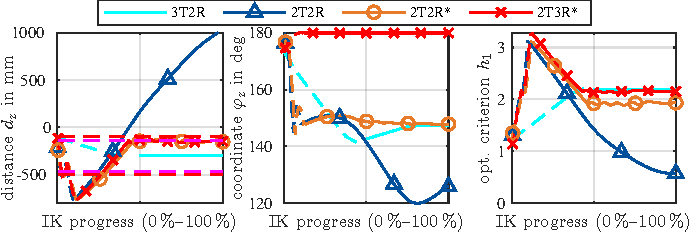
\includegraphics[]{figures/ik_results.pdf}
\vspace{-0.4cm}
\caption{(\textbf{a}) Target distance $d_z$ with threshold $d_{z,\mathrm{thr,min/max}}$ and limit $d_{z,\mathrm{min/max}}$, (\textbf{b}) end effector rotation $\varphi_z$ corresponding to $\ks{E}$ and (\textbf{c}) joint limit optimization criterion $h_1$ over the convergence of the IK algorithm. Dashed lines mark $\Res \napprox \vec{0}$}
\label{fig:ik_results}
\vspace{-0.6cm}
\end{center}
\end{figure}




In the 2T2R case, without limiting the coordinate $d_z$, the functional redundancy of degree two is used only for a far reaching elongation of the arm in Fig.~\ref{fig:robots_ik_results}c.
This strongly improves $h_1$, but is infeasible regarding collisions, singularities and possible process restrictions.
This is improved by the method 2T2R* which uses $h_1+h_\mathrm{dist}$ at the cost of a degraded $h_1$, see Fig.~\ref{fig:robots_ik_results}d.
Using a fixed orientation $\varphi_z$ with 2T3R* does not allow to improve $h_1$ further since the one degree of functional redundancy is already used for $h_\mathrm{dist}$ which is at it's limit as can also be seen in Fig.~\ref{fig:robots_ik_results}e.
Finally, for comparison, the case of 3T2R in Fig.~\ref{fig:robots_ik_results}b is included with a shifted $\ks{D}$ in the middle of $d_{z,\mathrm{min}}$ and $d_{z,\mathrm{max}}$, which allows optimization of $h_1$ to a poorer result than the other methods due to the reduced range of self-motion.
While the overall convergence of all methods is clear from Fig.~\ref{fig:ik_results}, a remaining problem is visible at the 2T3R* case. 
Leaving the linear approximation leads to oscillations in the nullspace motion between the criteria $h_\mathrm{dist}$ and $h_1$, i.e. a degraded convergence in the second half of the motion, which may be solved by further tuning of the damping parameters.

\vspace{-0.4cm}
\section{Conclusion and Remark on Parallel Robots}
\label{sec:conclusion}
\vspace{-0.2cm}

The proposed formulation for the definition of the inverse kinematics problem can be used for tasks with two translational degrees of freedom and spatial motion, especially 2T2R and 2T3R.
The method is targeted at a numeric implementation with an analytic derivation and can be embedded in larger frameworks, such as task-priority inverse kinematics of \cite{MoeAntTeePet2016}.
Extensions such as the limitation of the redundant coordinate with a projection method make it feasible in practical applications.

The minimal dimension of the residual and the elimination of dependent operational space coordinates allow an efficient transfer to gradient projection schemes for \emph{parallel robots with functional redundancy} to extend works like \cite{ChenMcIYi2003} and \cite{KoblerKotLexMaj2014} on 2T2R tasks.
The first leg chain's kinematic constraints then correspond to the residual $\ResR$ in this paper and the constraints of following leg chains have to be defined relative to the first, leading leg \cite{SchapplerTapOrt2019}.
%The resulting constraints formulation then again does not include the redundant coordinates.
The functionally redundant direct and inverse kinematics matrices (``Jacobians'') can then be obtained by differentiating the constraints. % w.r.t. the joint and minimal 2T2R platform coordinate $\vec{y}$ introduced in this paper.
The position-level IK can then be used for pose optimization in synthesis or control.


\begin{acknowledgement} % should be the start of page 8
The authors acknowledge the support by the Deutsche Forschungsgemeinschaft (DFG) under grant number 341489206. \textsc{Matlab} code to reproduce the results
is available at GitHub under free license at \url{github.com/SchapplM/robotics-paper_ark2022_2T2R}.
\end{acknowledgement}
\vspace{-0.9cm} % keep references on page 8
\renewcommand{\baselinestretch}{0.965} % compact references section
\bibliographystyle{spmpsci}
\bibliography{references}

\end{document}
